\documentclass{article}

%%%%%%%%%%%%%%%%%%%%%%%%%%%%%%%%%%%%%%%%%%%%%%%%%%%%%%%%%%%%%%%%%%%%%%%%%%%%%%%%
%%%  packages
%%%%%%%%%%%%%%%%%%%%%%%%%%%%%%%%%%%%%%%%%%%%%%%%%%%%%%%%%%%%%%%%%%%%%%%%%%%%%%%%
\usepackage[utf8]{inputenc}

\usepackage{graphicx}
\usepackage{hyperref}
\usepackage{cleveref}
\usepackage{xspace}
\usepackage{authblk}


%%%%%%%%%%%%%%%%%%%%%%%%%%%%%%%%%%%%%%%%%%%%%%%%%%%%%%%%%%%%%%%%%%%%%%%%%%%%%%%%
%%%  definitions
%%%%%%%%%%%%%%%%%%%%%%%%%%%%%%%%%%%%%%%%%%%%%%%%%%%%%%%%%%%%%%%%%%%%%%%%%%%%%%%%
\newcommand{\eg}{e.g.\ }
\providecommand{\email}[1]{\href{mailto:#1}{#1}}

%%%%%%%%%%%%%%%%%%%%%%%%%%%%%%%%%%%%%%%%%%%%%%%%%%%%%%%%%%%%%%%%%%%%%%%%%%%%%%%%
%%%  front matter
%%%%%%%%%%%%%%%%%%%%%%%%%%%%%%%%%%%%%%%%%%%%%%%%%%%%%%%%%%%%%%%%%%%%%%%%%%%%%%%%

\title{ICARUS TPC channel mapping}

% \author{
%   Biswaranjan Behera \thanks{Colorado State University, CO, U.S.A.; \email{biswaranjan.behera@colostate.edu}}
%   \and
%   Angela Fava \thanks{\email{afava@fnal.gov}}
%   \and
%   Gianluca Petrillo \thanks{\email{petrillo@slac.stanford.edu}}
%   \and
%   Filippo Varanini \thanks{\email{filippo.varanini@pd.infn.it}}
% }
%

\author[a]{Biswaranjan Behera \thanks{\email{biswaranjan.behera@colostate.edu}}}
\author[b]{Angela Fava \thanks{\email{afava@fnal.gov}}}
\author[c]{Gianluca Petrillo \thanks{\email{petrillo@slac.stanford.edu}}}
\author[d]{Filippo Varanini \thanks{\email{filippo.varanini@pd.infn.it}}}

\affil[a]{Colorado State University, Fort Collins, CO, U.S.A.}
\affil[b]{Fermi National Accelerator Laboratory, Batavia, IL, U.S.A.}
\affil[c]{SLAC National Accelerator Laboratory, Menlo Park, CA, U.S.A.}
\affil[d]{INFN Padova, Italy}

\date{\today}

%%%%%%%%%%%%%%%%%%%%%%%%%%%%%%%%%%%%%%%%%%%%%%%%%%%%%%%%%%%%%%%%%%%%%%%%%%%%%%%%
\begin{document}
%%%%%%%%%%%%%%%%%%%%%%%%%%%%%%%%%%%%%%%%%%%%%%%%%%%%%%%%%%%%%%%%%%%%%%%%%%%%%%%%
%%% title page
%%%%%%%%%%%%%%%%%%%%%%%%%%%%%%%%%%%%%%%%%%%%%%%%%%%%%%%%%%%%%%%%%%%%%%%%%%%%%%%%

\maketitle

\begin{abstract}
We describe the mapping between physical wires and readout channels in ICARUS
detector as installed at Fermilab,
including all the assumptions involved in the definition of the mapping.
\end{abstract}


%%%%%%%%%%%%%%%%%%%%%%%%%%%%%%%%%%%%%%%%%%%%%%%%%%%%%%%%%%%%%%%%%%%%%%%%%%%%%%%%


\section{Introduction}
\label{sec:intro}

This document describes the relation between physical TPC wires and readout
channels (\emph{channel mapping}), at the best of the current knowledge.

Precision of the language is capital when describing this mapping.
\Cref{sec:glossary} lists the technical names we use in the report.
Those definitions apply within this document even when they happen to be
different from the currently commonly used ones.



\section{Sources}
\label{sec:sources}

The mapping can be deduced based on the following information:
\begin{itemize}
  \item geometric information from ICARUS detector blueprints~\cite{SBNDocDB1020}
    (with the caveat that second induction and collection planes on one of the
    TPCs are swapped, see \cref{fig:WirePlanesInTPC})
  \item undocumented information on the cabling, reported in \cref{ssec:CablingInfo}
  \item information from the (currently unpublished) general technical note
    on the TPC connectivity test~\cite{SBNDocDBxxxx:ConnTest},
    replicated in \cref{ssec:PlaneAssignment}
\end{itemize}


\subsection{Cabling details}
\label{ssec:CablingInfo}

This information was provided by Angela Fava:
\begin{itemize}
  \item all cables are installed sequentially at the TPC end, and the wires within the flat cable are numbered following the same sequence;
  \item for Induction1 A1-33, B1-33, C1-33 and D-133 are all top to bottom (therefore the red conductor is at the top);
  \item for corners F1-17 and H1-17 are bottom to top, while E1-17 and K1-17 are top to bottom;
  \item please note that there is a mistake in Fig. 2 at page 7 in the tech note, in that the South-East corner is Collection and the North-East is Induction 2;
  \item for standard chimneys 1 to 9 and 10 to 18 SHOULD be North to South, but for cross-checking this I have asked photo documentation to Andrea Zani and Claudio and I am waiting on their reply.
\end{itemize}


\subsection{Assignment of wire planes to minicrate sides}
\label{ssec:PlaneAssignment}

\begin{figure}[p]
  \centerline{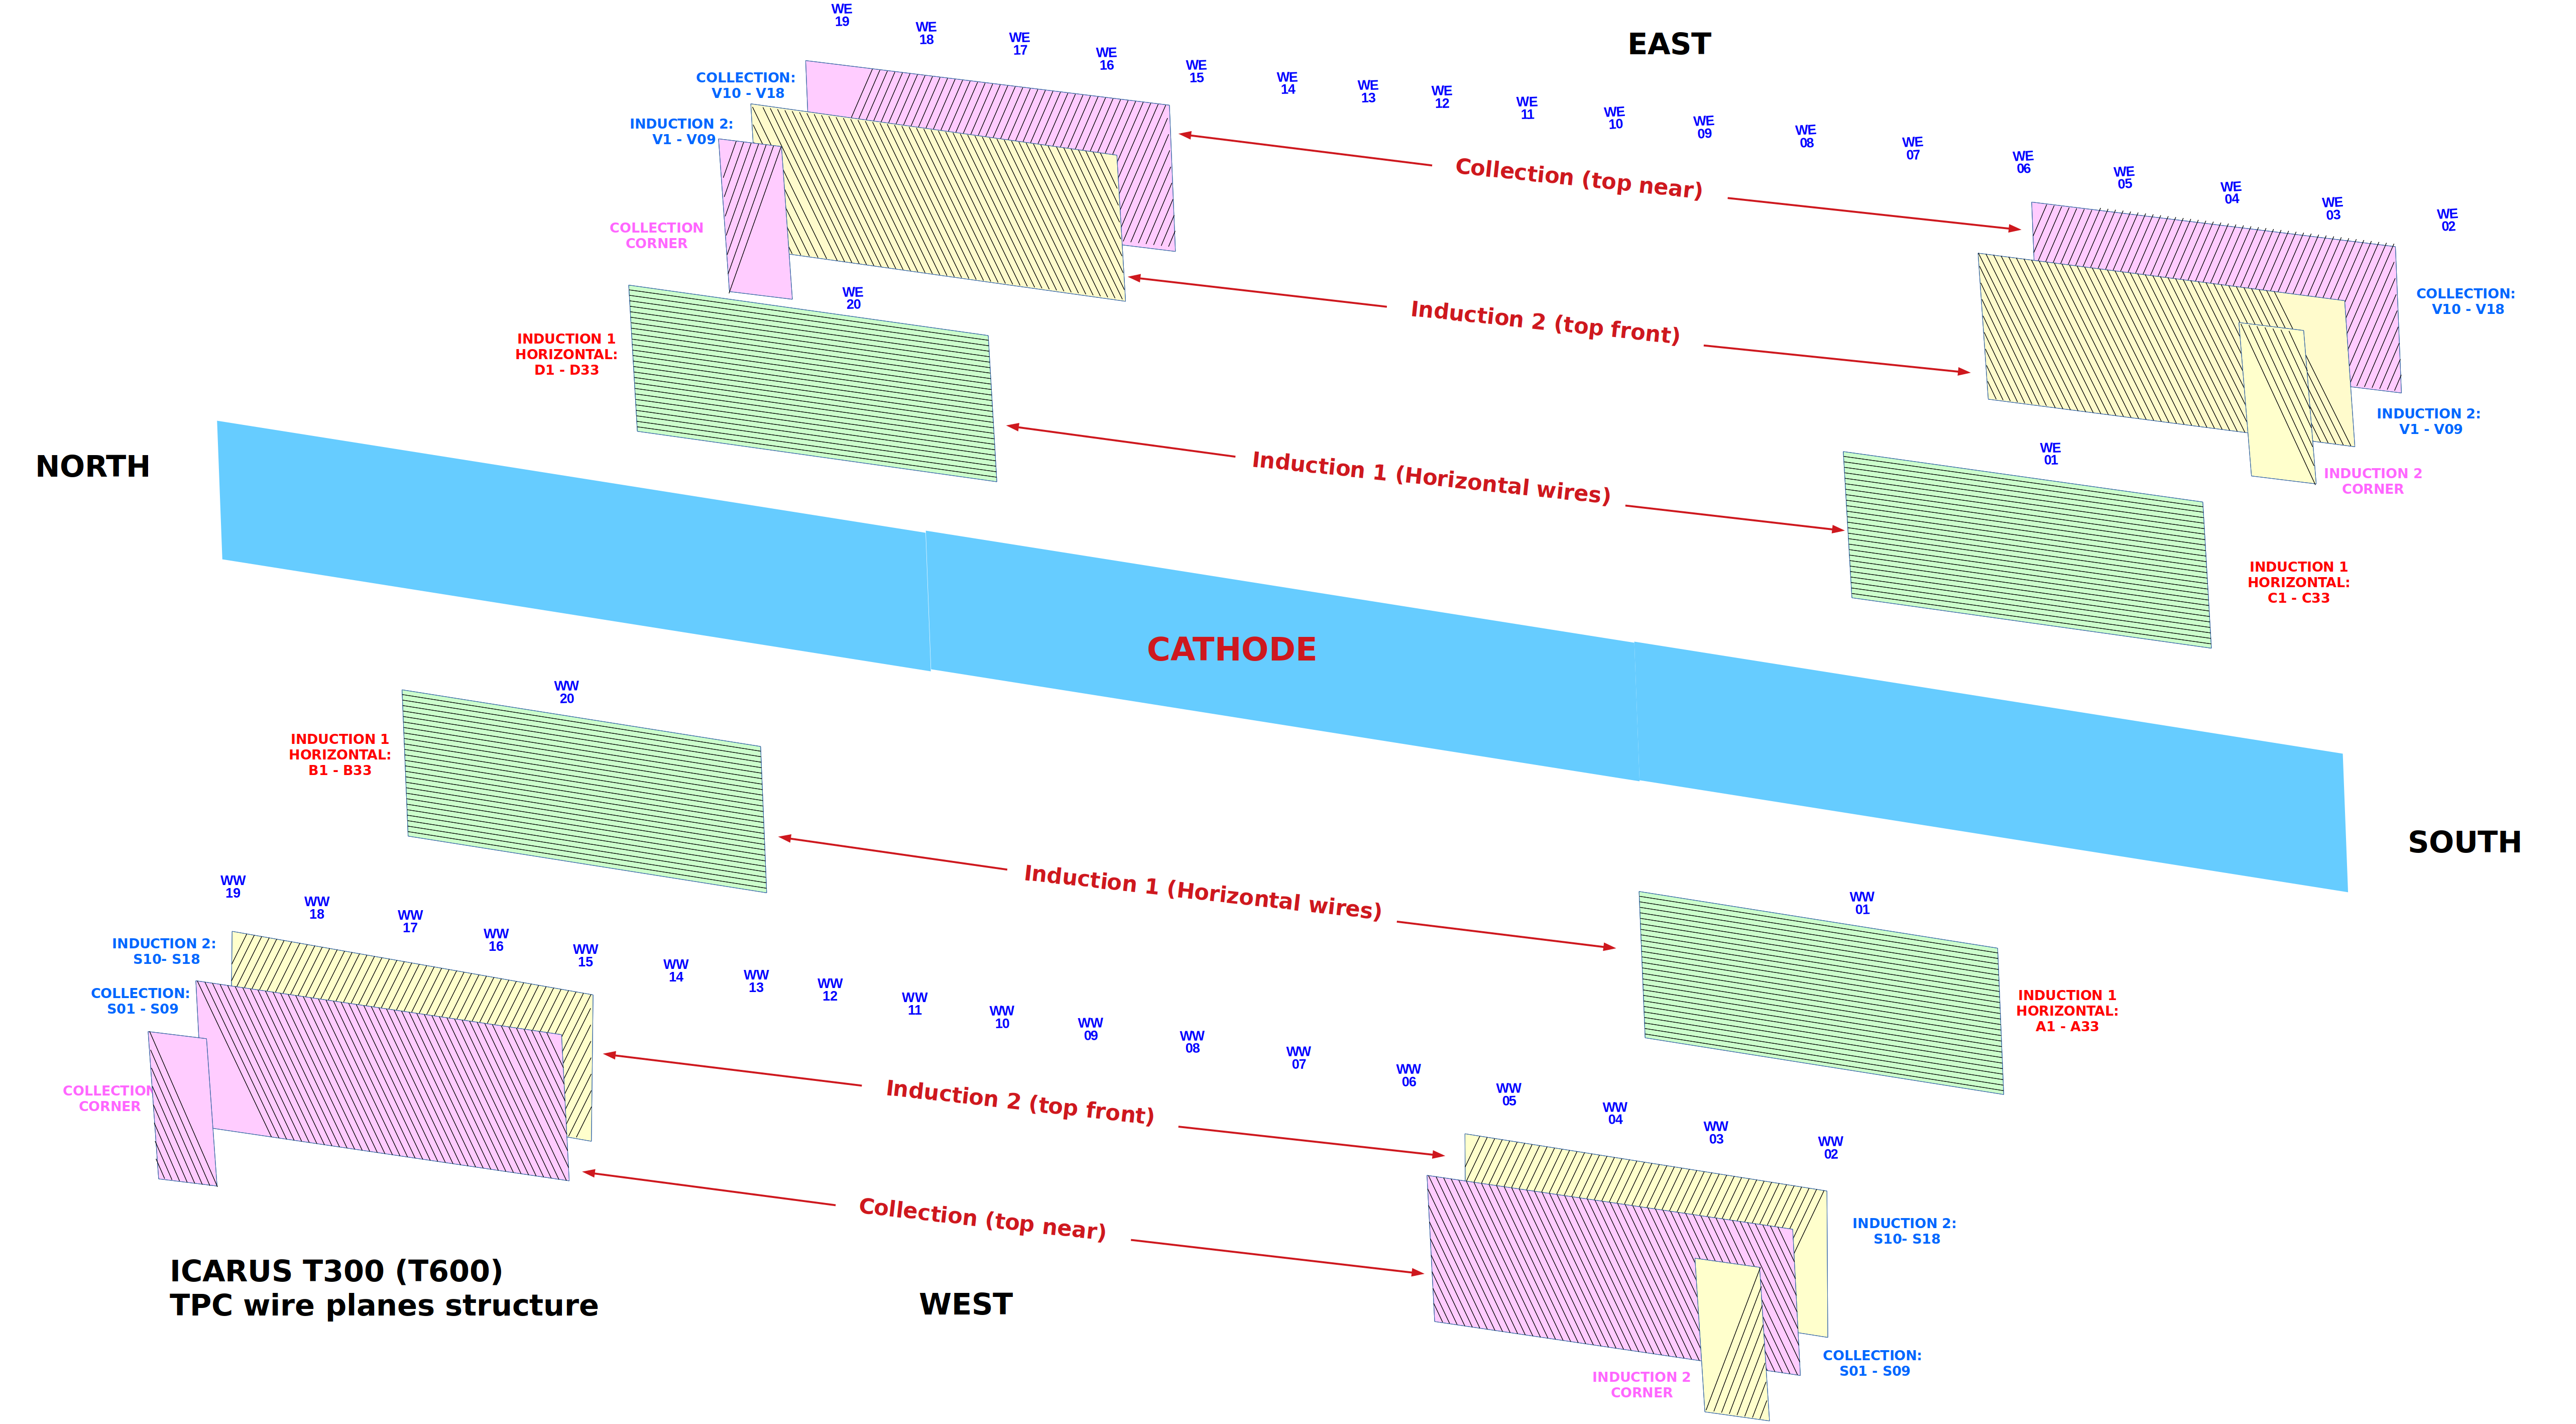
\includegraphics[width=0.8\textheight,angle=90]{figures/Icarus_TPC_wp}}
  \caption{
    Wire planes in a cryostat and their disposition (from~\cite{SBNDocDBxxxx:ConnTest}).
    Note the orientation of the wires, correct and contrasting with the erroneous one in~\cite{SBNDocDB1020}.
    \label{fig:WirePlanesInTPC}
  }
\end{figure}

This information is extracted from a technical note~\cite{SBNDocDBxxxx:ConnTest} describing the TPC connectivity test:
\begin{itemize}
  \item in chimneys WW and EW:
    \begin{itemize}
      \item flat cables from 1 to 9 are connected to wires on the \emph{collection plane}
      \item flat cables from 10 to 18 are connected to wires on the \emph{second induction plane}
    \end{itemize}
  \item in chimneys WE and EE:
    \begin{itemize}
      \item flat cables from 1 to 9 are connected to wires on the \emph{second induction plane}
      \item flat cables from 10 to 18 are connected to wires on the \emph{collection plane}
    \end{itemize}
\end{itemize}



%%%%%%%%%%%%%%%%%%%%%%%%%%%%%%%%%%%%%%%%%%%%%%%%%%%%%%%%%%%%%%%%%%%%%%%%%%%%%%%%
\section{Glossary}
\label{sec:glossary}

\begin{description}
  \item[collection plane] is the wire plane farthest from the cathode,
    with most of the wires read on top of the anode frame and a few read on one
    of the anode frame sides
  \item[first induction plane] is the wire plane closest to the cathode,
    with 9-meter long wires being read out on the sides of the anode frame
  \item[flange] one of the 96 interfaces between cold and warm volumes
    \emph{serving the TPC wire planes}
    (other flanges, \eg the ones serving the photomultipliers, are never
    considered in this document)
  \item[flat cable] each of the 68-wire twisted-pair cables connecting one side
    of the decoupling and biasing board to a group of 32 contiguous TPC wires
    at the anode frame
  \item[minicrate] metal crate hosting nine readout boards,
    and installed on the warm side of each of the 96 flanges.
  \item[second induction plane] is the middle wire plane,
    with most of the wires read on top of the anode frame and a few read on one
    of the anode frame sides
\end{description}


%%%%%%%%%%%%%%%%%%%%%%%%%%%%%%%%%%%%%%%%%%%%%%%%%%%%%%%%%%%%%%%%%%%%%%%%%%%%%%%%
%%% bibliography
%%%%%%%%%%%%%%%%%%%%%%%%%%%%%%%%%%%%%%%%%%%%%%%%%%%%%%%%%%%%%%%%%%%%%%%%%%%%%%%%
\bibliographystyle{abbrv}
\bibliography{ICARUS}

%%%%%%%%%%%%%%%%%%%%%%%%%%%%%%%%%%%%%%%%%%%%%%%%%%%%%%%%%%%%%%%%%%%%%%%%%%%%%%%%
%%% that's it
%%%%%%%%%%%%%%%%%%%%%%%%%%%%%%%%%%%%%%%%%%%%%%%%%%%%%%%%%%%%%%%%%%%%%%%%%%%%%%%%

\end{document}
%%%%%%%%%%%%%%%%%%%%%%%%%%%%%%%%%%%%%%%%%%%%%%%%%%%%%%%%%%%%%%%%%%%%%%%%%%%%%%%%
